\section{2c: Interrupts}
The solution of our previous problem is interrupts! Instead of waiting for each I/O to responds, we can do our work and \important{when a I/O} \textit{shouts} we do what he want us to do. We have them \important{ask} for \important{attention}\\
\begin{parag}{Seen this already in some languages}
	We maybe, have already seen this mecanics in some languages:
	\begin{itemize}
	    \item Callbacks, Action, or \important{Event Listeners} (PPO), signals, promises, Futures, Hooks
	\end{itemize}
	However does are done by the \important{compiler}/ \important{interpreters}. Here, we are dealing with the cpu directly so how can we do this?
\end{parag}
\begin{parag}{The basic Idea of I/O interrupts}
    \begin{center}
    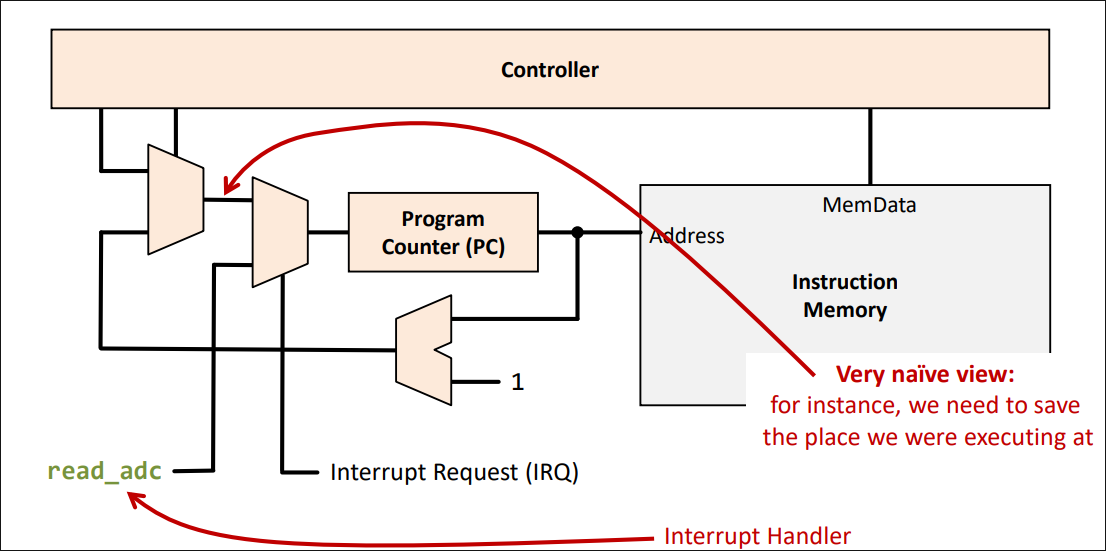
\includegraphics[scale=0.3]{screenshots/2025-10-22_12.png}
    \end{center}
	We use the \texttt{read\_adc} address which is where we handle the I/O interrups. The interrupt request serve to trigger the interruption.\\
	However the is several issues to take care of and behaviours to define:
	\begin{itemize}
	    \item We need to know \important{who needs attention} -- we do not have only one peripheral
			\begin{itemize}
				\item After interrupt, \important{the software checks all peripherals} in turn (polling), or 
				\item \important{I/O peripheral sends identification}
			\end{itemize}
		\item \important{Different priorities} need to be expressed -- some peripheral can wait long, some cannot
		\item \important{Impact on current execution}: Current instruction(s) can complete? One? Five? Twenty? What ahhpens of the program that was executing?
	\end{itemize}
	\begin{subparag}{How do many peripheral connect to a single IRQ}
	    In order to do so, we have more than one way, the easiest and most intuitive is a or with $n$ inputs.\\
		On the other hand, what we also can do is to use tri-state buffers, one for each IRQ$_n$.
	\end{subparag}
	\begin{center}
	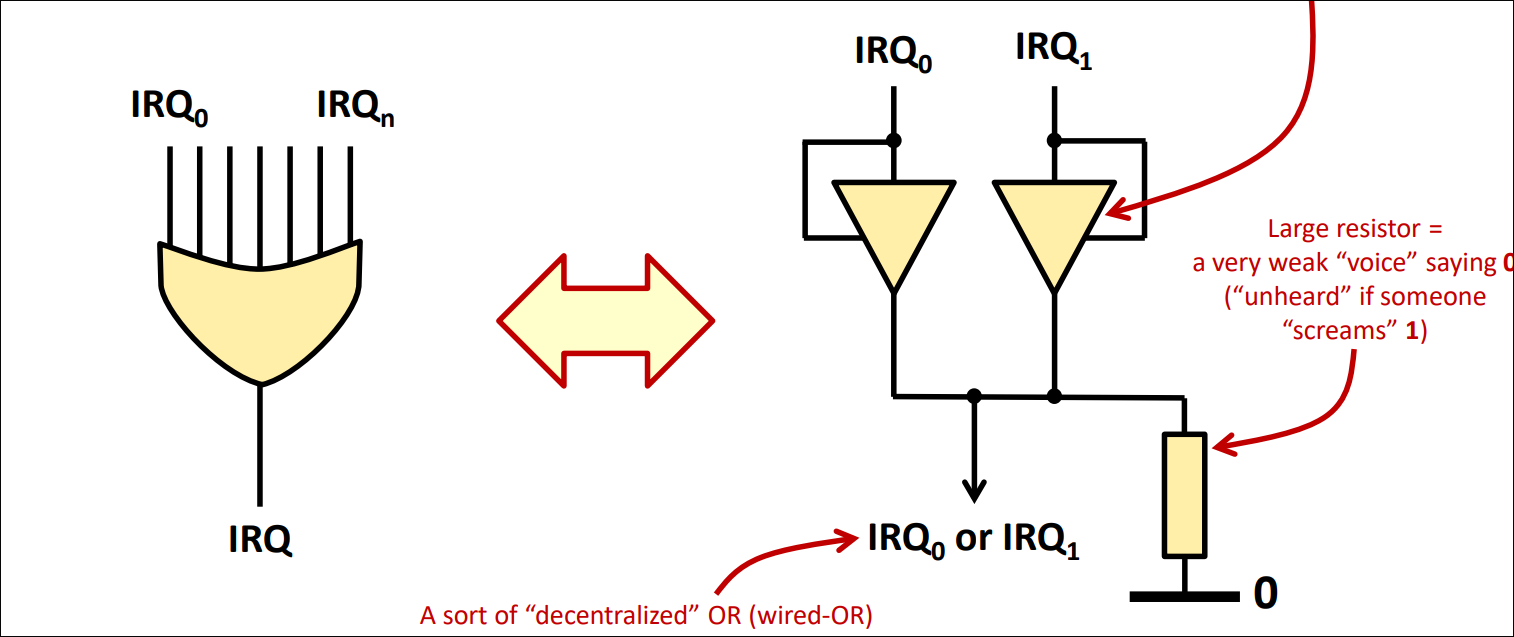
\includegraphics[scale=0.2]{screenshots/2025-10-22_13.png}
	\end{center}
	\begin{subparag}{Example sequence}:
	    \begin{enumerate}
	        \item peripheral asks for attention through IREQ
	        \item Processor signals when it is ready to serve peripheral through IACK "\textit{acknowledges}" the interrupt)
	        \item peripheral signals its identity
	        \item Processor takes appropriate action --transfer control to the appropriate Exception handler
	        \item Processor reverts to the interrupt task
	    \end{enumerate}
	
	\end{subparag}
\end{parag}
		\begin{figure}[h!]
		    \centering
			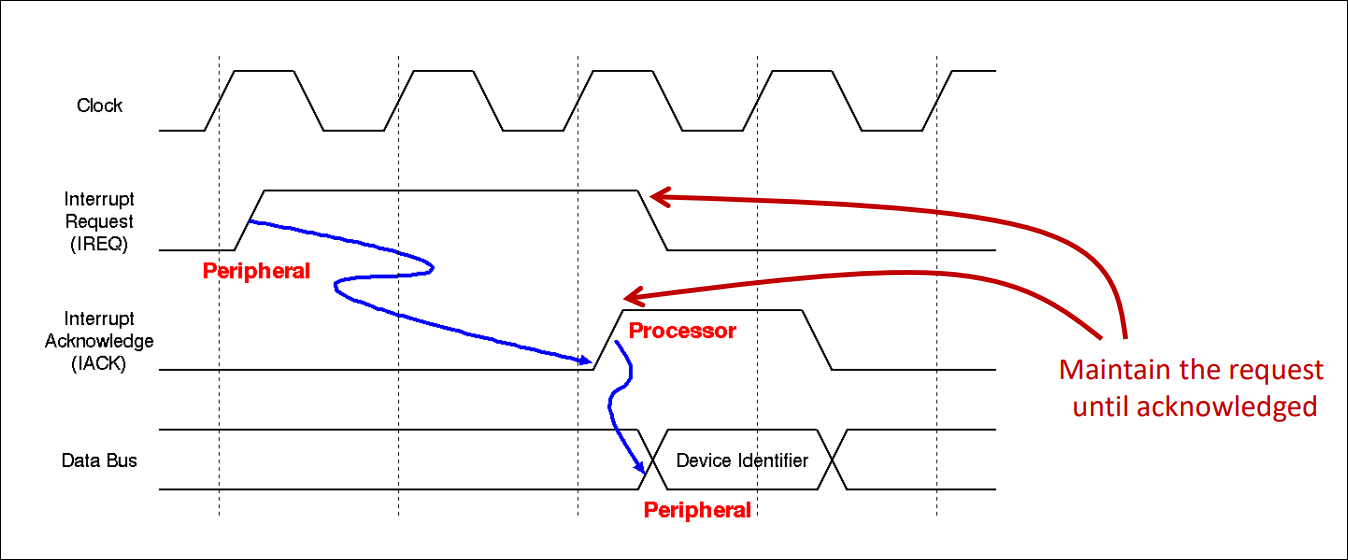
\includegraphics[scale=0.2]{screenshots/2025-10-22_14.png}
			\caption{tiaming diagram}
		\end{figure}
\begin{framedremark}
	On the software side, it works with the same code we used before for polling. However, the \texttt{read\_adc} function is now called by the interrupt handler. The interrupt handler stores the address of the program that manages all interrupt requests, and from there, it launches the program that handles the ADC.
\end{framedremark}
\begin{framedremark}
It is a very good practice to just look at the timing diagram and "\textit{guess}" how the circuit would look like.
\end{framedremark}
\begin{parag}{I/O Interrupt priorities}
    \important{Daisy chain arbitration} is one of the simplest methods:
	\begin{itemize}
	    \item Anyone places request (IREQ, Request)
	    \item Acknowledge line (IACK, Grant) passed from one device to the next 
	    \item Device which wants access, intercepts the signal and hides it from successice devices 
	    \item Simple but (1) slow and (2) hard priorities (meaning hard in like hardcode something).
	\end{itemize}
	\begin{center}
	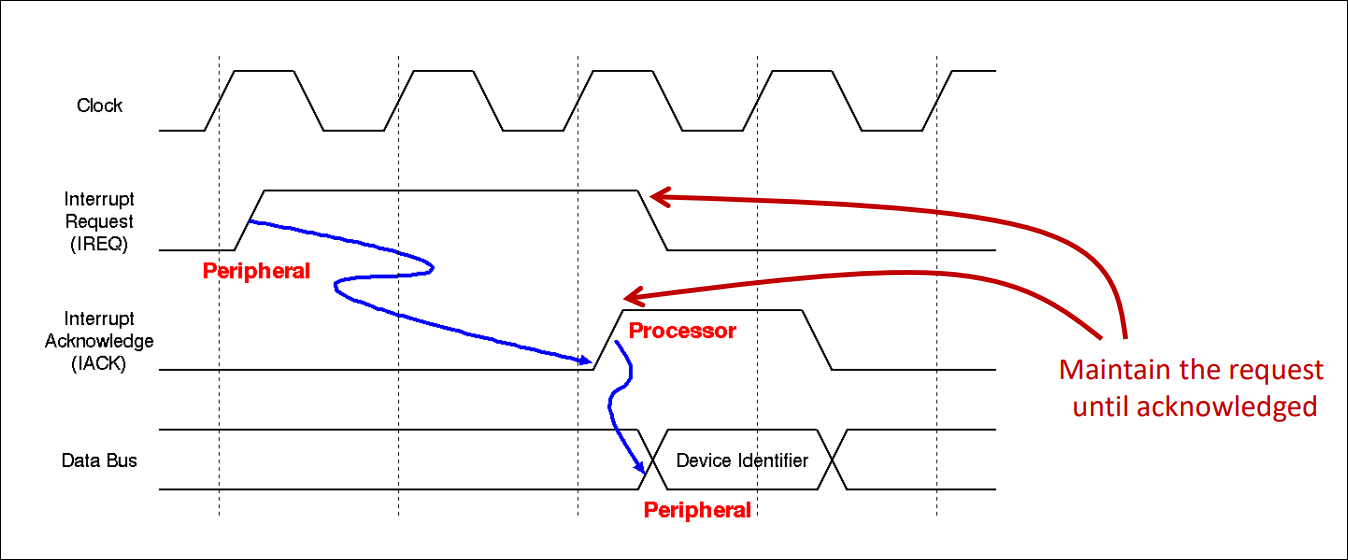
\includegraphics[scale=0.2]{screenshots/2025-10-22_14.png}
	\end{center}
\end{parag}
\begin{parag}{Interrup controller}
	More sophisticated methods involve special hardware:\\
	An \important{interrupt controller}  may be expected to:
	\begin{itemize}
		\item Propagate only one \texttt{IREQ} at a time to the processor 
			\begin{itemize}
			    \item Select the one with highest fixed priority
			    \item Select the one with equal priority which has been served last.
			\end{itemize}
			\item Propagate the returned \texttt{IACK} to the appropriate peripheral
			\item Inhibit certain devices from sending \texttt{IREQ}s 
			\item Allow nesting, that is higher priority \texttt{IREQ} to propagate while lower priority interrupts are being served.
	\end{itemize}
	\begin{center}
	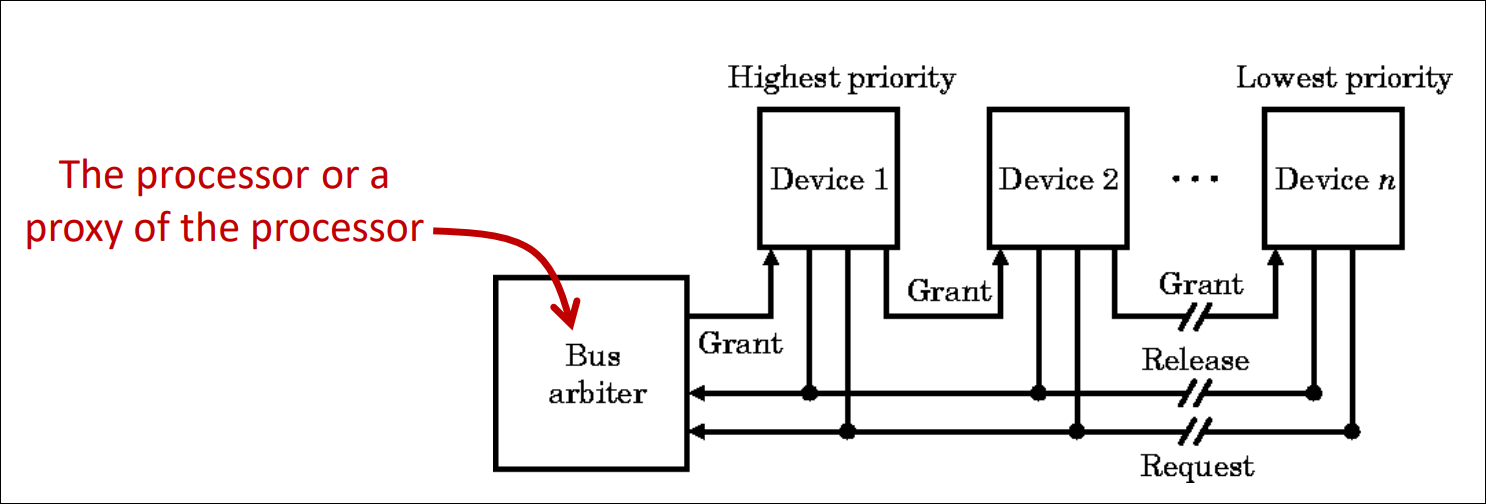
\includegraphics[scale=0.2]{screenshots/2025-10-22_15.png}
	\end{center}
\end{parag}

\subsection{Direct Memory Access (DMA)}

Even when using interrupts, the processor can spend a significant amount of time transferring data to and from input/output devices. This is especially problematic when dealing with high-throughput peripherals such as disks or network interfaces, where large amounts of data need to be moved. To address this inefficiency, the concept of Direct Memory Access (DMA) is introduced. With DMA, a dedicated hardware peripheral takes over the task of transferring data between memory and the I/O devices. This allows the CPU to continue executing other instructions while the data transfer occurs in parallel. By offloading these memory operations to the DMA controller, overall system performance is improved, and the CPU is no longer tied up managing large data transfers.\\
This idea shortly is:
\begin{itemize}
	\item Let’s have a \important{special peripheral} perform the needed data transfers from and to memory (R/W) and free the processor to continue computation
\end{itemize}
\begin{parag}{Without DMA}
    What we used to do before is:
	\begin{enumerate}
	    \item The peripheral launch a interrupt request
	    \item The Processor load the data from the peripheral
	    \item The processor store the data into the memory
	\end{enumerate}
	This processor can be done for like 1,000,00 times.
\end{parag}
\begin{parag}{With the DMA}
    The idea now is to:
	\begin{enumerate}
	    \item The peripheral launch a interrupt request
	    \item The processor launch it back to the DMA (with the needed informations)
	    \item The DMA load 
	    \item The DMA store it to the memory
	\end{enumerate}
	We do the same thing as before except the \textit{boring} part of load store, load, store, load, store ... is done by the DMA.
	\begin{center}
	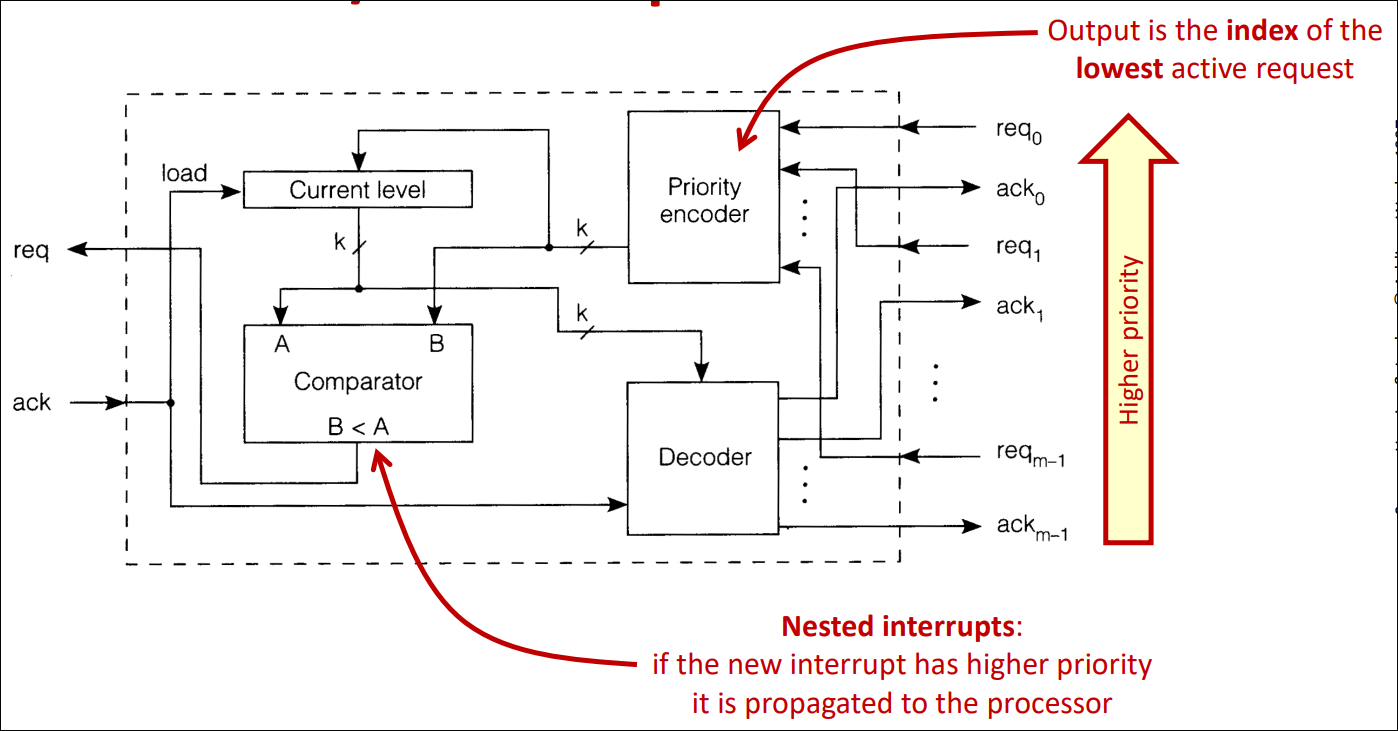
\includegraphics[scale=0.2]{screenshots/2025-10-22_16.png}
	\end{center}
	\begin{framedremark}
	I put only one screen here but there were like a nice way of introducing it in the slide so I'll just say it there, this is the 2.c. interrupts slide 14 to 24.
	\end{framedremark}
\end{parag}
\begin{parag}{Direct Memory Access}
   \begin{definition}
   A minimal DMA is:
   \begin{itemize}
       \item An \important{increment register} (how many bytes/words to transfer at a time)
       \item A couple of \important{address pointers} (source address pointer and destination address pointer), incremented by the above constant at every transfer 
       \item A \important{counter} (total number of bytes/words to transfer).
   \end{itemize}
   \end{definition} 
   \begin{subparag}{Example}
       Here an example of a sequence:
	   \begin{enumerate}
	       \item The processor tells the DMA controller (a) which device to access, (b) where to read or write the memory, and (c) the number of bytes to transer.
	       \item The DMA controller becomes bus master and performs the required accessses controlling directly the address and control busses.
	       \item The DMA controller sends an interrupt to the processor to signal succesful completion or erros
	   \end{enumerate}
	   
   \end{subparag}
\end{parag}



\begin{parag}{Timer and Periodic DMA Operations}
    In some cases, we want DMA transfers to happen at regular intervals without the CPU constantly supervising them. This is where a \important{timer} comes in. A timer is a hardware peripheral that counts up (or down) automatically and can generate an \important{interrupt} when it reaches a programmable maximum value. By configuring a timer, the CPU can schedule periodic DMA operations, such as reading data from a sensor every millisecond or streaming data from a peripheral continuously. This mechanism allows the DMA to start transfers on its own, triggered by the timer interrupt, freeing the CPU from constantly checking or initiating these operations.
\end{parag}

\begin{parag}{Bus Control and Processor Cooperation}
    During a DMA transfer, the DMA controller must temporarily take control of the memory bus, becoming the \important{bus master}. The processor must \important{relinquish control of the bus} during this period, but it can continue executing instructions that do not require bus access, such as computations using registers. Once the DMA completes the transfer, it sends an interrupt to the processor to signal successful completion or report any errors. This cooperation ensures that both CPU and DMA operate efficiently without conflicts on the memory bus.
\end{parag}

\begin{parag}{Advantages of DMA}
    Using DMA brings several benefits to a system:
    \begin{itemize}
        \item It offloads repetitive memory transfer tasks from the CPU, reducing workload.
        \item It increases system throughput, especially for large data blocks from high-speed peripherals.
        \item It allows the CPU to focus on computation or other tasks while data transfers happen in parallel.
        \item It reduces the time the CPU spends in \important{busy-waiting} loops checking for I/O readiness.
    \end{itemize}
\end{parag}

\begin{parag}{Example Sequence with Timer and DMA}
    An example sequence of operations with a timer and DMA could be:
    \begin{enumerate}
        \item The timer reaches its programmed max value and generates an interrupt.
        \item The processor acknowledges the timer interrupt and instructs the DMA controller to start a transfer from a peripheral to memory.
        \item The DMA controller becomes the bus master and performs the required memory accesses, reading from the peripheral and storing into memory.
        \item Once the transfer is complete, the DMA sends an interrupt to the processor to indicate completion.
        \item The CPU resumes normal execution, potentially until the next timer-triggered DMA transfer.
    \end{enumerate}
    This sequence illustrates how CPU, DMA, timer, and peripherals interact to efficiently handle high-throughput data transfers.
\end{parag}






